\documentclass{scrreprt}
\usepackage{enumitem}
\usepackage{listings}
\usepackage{underscore}
\usepackage{graphicx}
\usepackage{float}
\usepackage{tabularx}
\usepackage[bookmarks=true]{hyperref}
\usepackage[utf8]{inputenc}
\usepackage[english]{babel}
\def\myversion{1.0 }
\graphicspath{ {./figures/} }
\date{}
%\title
\usepackage{hyperref}
\begin{document}

\begin{flushright}
    \rule{16cm}{5pt}\vskip1cm
    \begin{bfseries}
        \Huge{SOFTWARE REQUIREMENTS\\ SPECIFICATION}\\
        \vspace{1.5cm}
        for\\
        \vspace{1.5cm}
        WELCOMEX\\
        \vspace{1.5cm}
        \LARGE{Version \myversion}\\
        \vspace{1.5cm}
        Prepared by :  \\
        Andrea Michel Quintero Montalvo\\
        Bryan Santiago Mora Molina\\
        María del Carmen González García\\
        Ricardo Nieto Padilla\\
        Roberto Ortíz Monroy\\
        \vspace{1.5cm}
        Submitted to : Ray Brunet Parra Galaviz \\Lecturer\\
        \vspace{1.5cm}
    \end{bfseries}
\end{flushright}

\tableofcontents

\listoffigures

\chapter{Introduction}

\section{Purpose}
The purpose of this document is to provide an extensive and detailed overview of the requirements necessary for the development of the Welcomex software. This comprehensive document is intended to make clear the scope of the project and its objectives.

Moreover, this document will cover in detail the system's constraints, highlighting any limitations or restrictions that might impact the development process or the final product's functionality. It will also delve into the system's interface design, offering insights into how users will interact with the software and the overall user experience envisioned by the development team.

Additionally, this document will address the software's interactions with other external applications, providing a clear description of how Welcomex will integrate with and communicate with these systems. This section will outline the necessary protocols, data exchange formats, and interfaces that will enable seamless interoperability between Welcomex and other software, ensuring that the system can function effectively within the broader digital ecosystem.

Through a thorough examination of these components, this document serves as a foundational blueprint for the Welcomex software development project. It is intended to guide the development team in creating a product that meets the specified requirements and expectations.
\section{Project Scope}
The Welcomex software is a web-based platform designed to facilitate the registration and analysis of migration statistics in Mexico. This project aims to serve as a dedicated tool for the efficient collection of relevant data and the comprehensive analysis of the country's migratory situation. Welcomex would be able to provide insightful statistical data on migrants, such as reasons for migration, age, gender, socioeconomic status, and more. This information will enable a clearer understanding of the needs of migrants, aiding in the provision of necessary supplies and support at shelters.

The primary purpose of Welcomex is to enhance the understanding and management of migration phenomena in Mexico more effectively. The software seeks to facilitate communication among stakeholders involved in migration management; provide peace of mind to those concerned about migration patterns and impacts; and enable the visualization of migration data in a user-friendly manner.

These objectives align with the broader goal of improving decision-making processes, offering targeted support to the migrant population, and contributing to research efforts. Welcomex aims to be an integral tool that supports continuous monitoring, promotes transparency, and aids in achieving national and international migration-related goals.

\section{Definitions, acronyms, and abbreviations}
\setlength{\arrayrulewidth}{0.5mm}
\setlength{\tabcolsep}{18pt}
\renewcommand{\arraystretch}{1.5}
\begin{tabular}{ |p{3cm}|p{9cm}|}
 \hline
  Term & Definition\\
 \hline
 Progressive Web Application & A progressive web app (PWA) is an app that's built using web platform technologies, but that provides a user experience like that of a platform-specific app.\\
 \hline
 API & An API, which stands for application programming interface, is a set of protocols that enable different software components to communicate and transfer data. \\
 \hline
 Database & A database is an organized collection of structured information, or data, typically stored electronically in a computer system.\\
  \hline
 AWS & Amazon Web Services (AWS) is the world’s most comprehensive and broadly adopted cloud, with more than 200 fully featured services available from data centers globally.\\
 \hline
 AWS Rekognition & Amazon Rekognition is a service that makes it easy to add powerful visual analytics to your applications. Rekognition Image allows you to create powerful applications for searching, verifying and organizing millions of images.\\
\hline
 AWS S3 & Amazon Simple Storage Service (Amazon S3) is an object storage service that offers industry-leading scalability, data availability, security, and performance.\\
 \hline
\end{tabular}

\section{References}








\chapter{Overall Description}
\section{Product Perspective}
The Welcomex software system is conceptualized as a comprehensive solution designed to address the complexities of managing and analyzing migration statistics in Mexico.  Welcomex is not recognized as an ongoing part of a product family or as a substitute for current systems; instead, it establishes itself as a wholly new solution within the social market it targets. Prior research indicates that no similar offerings exist, thereby affirming the system's uniqueness and innovation.

This system is designed as a comprehensive system comprising a Progressive Web Application (PWA), an Application Programming Interface (API), and a robust database, all of which are integrated with various Amazon Web Services for enhanced functionality.

The PWA is the front end of the system, accessible to users on various devices, offering a seamless and responsive interface for data registration and analysis. It interacts directly with the API, which acts as the middle layer facilitating communication between the front end and the database. It processes requests, executes business logic, interacts with the database for data storage and retrieval.

AWS Rekognition is utilized for facial recognition features within the PWA, allowing for advanced analysis and identification tasks. This service enhances the system's capabilities in processing and analyzing images related to migration data. Furthermore, this service will be integrated alongside AWS S3, which serves as a repository for storing images and other documents uploaded to the system. It provides a secure and scalable storage solution, ensuring that data is accessible and managed efficiently.

\section{Product Functions}
Within the Welcomex system, a range of functions have been meticulously designed to address the multifaceted needs of migration management and support. At the core of its functionalities is the ability to consult and manage detailed dashboards that display insightful graphs and statistics related to migrants and shelters. These dashboards are crafted to provide users with a comprehensive and intuitive overview of the migration landscape, including demographic trends, patterns of movement, and the status of shelters. This feature enables stakeholders to make informed decisions, assess the impact of migration, and plan resources and support more effectively.

In addition to the analytical capabilities, Welcomex offers robust tools for consulting and managing migrant data. Users can access individual profiles, update information, and track the migration journey of individuals. This aspect of the system is crucial for maintaining accurate and up-to-date records, facilitating the provision of targeted support and services to the migrant population.

A pivotal function of the Welcomex system is its ability to register visits of migrants to shelters. This process is streamlined through multiple entry points: searching for an individual by name, employing facial recognition technology to identify the person, or registering a new profile if the individual is not found in the system. This flexibility ensures that the registration process is inclusive and efficient, catering to the diverse circumstances of migrants seeking shelter. The integration of facial recognition technology, in particular, underscores the system's commitment to leveraging advanced technological solutions to enhance service delivery and operational efficiency.

Furthermore, the system encompasses a comprehensive module for managing the inventory of shelters. This function allows shelter administrators to keep track of supplies, manage stock levels, and identify needs in real time. By ensuring that the storage of shelters is well-organized and responsive to the changing needs of the migrant population, Welcomex plays a vital role in enhancing the capacity of shelters to provide for their inhabitants.

Overall, the Welcomex system is designed as an all-encompassing platform that not only facilitates the efficient management of migration-related data but also empowers users to provide meaningful support to migrants and shelters. Through its sophisticated dashboards, data management tools, registration capabilities, and inventory management features, Welcomex stands as a testament to the potential of technology to make a significant impact on social issues.

\section{User Classes and Characteristics}
The Welcomex system is designed to cater to a diverse user base, each with distinct roles and requirements, reflecting the multifaceted nature of migration management and support. At the heart of this ecosystem are three primary classes of users: shelter managers, shelter employees, and the general community, encompassing both families of migrants and researchers interested in migration data.

Shelter managers play a pivotal role within the Welcomex system, overseeing the operation of shelters and ensuring that they run smoothly and efficiently. These users leverage the system to gain a macroscopic view of shelter operations, including the management of supplies, the coordination of support services, and the monitoring of occupancy rates. Their interaction with the system is strategic, focusing on decision-making and resource allocation to enhance the welfare of migrants under their care. The functionality of the system enables these managers to maintain a high level of preparedness and responsiveness to the dynamic needs of the migrant population.

On the front lines of data entry and day-to-day operations are the shelter employees. These users are responsible for the majority of the important information entered into the Welcomex system, including registering visits of migrants to shelters through various means such as name searches, facial recognition, or new registrations. Their work is critical in maintaining up-to-date and accurate records of migrants, facilitating an organized and effective response to their needs. The system's user-friendly interface and streamlined processes are designed to minimize the administrative burden on these employees, allowing them to dedicate more time to direct support and assistance to migrants.

The general community represents a broad and diverse group of users, including families seeking information about relatives who have migrated and researchers looking to analyze migration patterns and statistics. For families, the Welcomex system provides a vital link to their loved ones, offering a way to track their journey and ensure their safety. This aspect of the system underscores its role in facilitating communication and peace of mind among those affected by migration. Meanwhile, researchers find in Welcomex a rich repository of data that can be used to study migration trends, inform policy-making, and contribute to the broader understanding of migration dynamics. The system's open access to anonymized data ensures that it serves as a valuable resource for academic and policy research while respecting the privacy and dignity of migrants.

Together, these user classes form a comprehensive ecosystem, each interacting with the Welcomex system in ways that reflect their unique needs and contributions to the field of migration support and management. The system's design is a testament to the importance of inclusivity and accessibility, ensuring that whether one is managing a shelter, inputting critical data, or seeking information on a loved one or research topic, the Welcomex system provides the necessary tools and resources to support their endeavors.

\section{Operating Environment}
The Welcomex software is designed to operate within a highly versatile and scalable digital environment, ensuring broad accessibility and compatibility with a range of hardware and software configurations. This adaptability is crucial for meeting the diverse needs of its users, from shelter managers and employees to the general community including families of migrants and researchers.
\subsection*{Hardware Platform}
Welcomex is primarily deployed as a Progressive Web Application (PWA), which means it is designed to work across a wide spectrum of devices including desktop computers, laptops, tablets, and smartphones. This approach ensures that users can access the system regardless of their hardware preferences, with the only requirement being a device capable of running a modern web browser. The system's responsive design adapts to different screen sizes and resolutions, providing an optimal user experience across all devices.
\subsection*{Operating System and Versions}
Given its web-based nature, Welcomex is operating system agnostic. It is accessible from any OS that can run a contemporary web browser, including but not limited to Windows, macOS, Linux, iOS, and Android. This broad compatibility ensures that the system is available to users with diverse technological resources and preferences, facilitating widespread adoption and use.
\subsection*{Software Components and Applications}
Welcomex's operation is supported by a backend infrastructure hosted on cloud services, specifically leveraging Amazon Web Services (AWS) for various functionalities including data storage (using AWS S3), and facial recognition capabilities (using AWS Recognition). The choice of AWS as a cloud provider ensures high availability, scalability, and security of the system's data and operations.

The system is designed to coexist peacefully with other software components and applications. On the user's end, it requires only a web browser such as Google Chrome, Mozilla Firefox, Microsoft Edge, or Safari for access. Its API architecture allows for integration with other systems, enabling data exchange and interoperability without disrupting existing workflows or software ecosystems that users might rely on. This includes potential integrations with governmental databases, research tools, or other relevant applications, ensuring Welcomex can function as part of a broader digital infrastructure for migration management and support.

In summary, the Welcomex software is engineered to operate within a diverse and inclusive technological environment, emphasizing ease of access, user-friendliness, and integration capability. Its design acknowledges the varied technological landscapes of its users, aiming to remove barriers to access and facilitate a seamless user experience across different platforms and devices.

\section{Design and Implementation Constraints}
The design and implementation of the Welcomex system are subject to a series of constraints that influence the range of options available to developers. These constraints stem from various sources including corporate policies, regulatory requirements, technological limitations, and operational considerations. Understanding these constraints is crucial for ensuring that the system is developed in a manner that meets all necessary standards and requirements, while also aligning with the project's overarching goals.
\subsection*{Corporate and Regulatory Policies}
Welcomex must comply with data protection and privacy laws relevant to the regions it operates in. This compliance affects how personal data is collected, stored, processed, and shared, requiring robust data protection measures and user consent mechanisms to be integrated into the system.
\subsection*{Hardware Limitations}
Given that Welcomex is a Progressive Web Application (PWA), the system is designed to be lightweight and efficient, minimizing hardware demands on the user end. However, developers must consider the variability in device capabilities among users, including differences in processing power, memory, and internet connectivity. These factors require optimization of the application's performance to ensure functionality across a broad range of devices.
\subsection*{Security}
Welcomex must incorporate comprehensive security measures to protect against unauthorized access, data breaches, and other cyber threats. This includes implementing authentication, authorization, data encryption, and regular security audits. Compliance with security standards and regulations is a non-negotiable aspect of the system's development.

\section{Assumptions and Dependencies}
In the development of the Welcomex system, certain assumptions and dependencies play a critical role in shaping the requirements and guiding the project's trajectory. Acknowledging these factors is essential for mitigating risks and ensuring that the system's development aligns with the project goals and user needs.

\begin{itemize}
    \item It is assumed that the target user base will have access to devices capable of running a modern web browser, allowing them to access the Progressive Web Application (PWA) without significant barriers. This assumption affects design decisions related to the application's complexity and usability.
    \item The system assumes reliable internet connectivity for users to access the web-based platform and for real-time data exchange with the cloud services and external APIs. This assumption influences the system's online functionalities and its reliance on cloud services.
    \item The system assumes a certain level of technical proficiency among users, particularly those responsible for data entry and management, such as shelter employees. This assumption impacts the design of the user interface and the complexity of user interactions.
\end{itemize}

\chapter{External Interface Requirements}
\section{User Interfaces}
The Welcomex system is designed with user experience at its forefront, ensuring that the interface is intuitive, accessible, and efficient for all user classes. The user interfaces are crafted to cater to the diverse needs of shelter managers, shelter employees, and the general community, each with distinct interactions with the system. While detailed user interface designs are documented separately, the following outlines the logical characteristics and standards guiding the user interface development.

The interface must be responsive, ensuring usability across a wide range of devices, from desktop computers to smartphones. This design approach facilitates access in various contexts, reflecting the diverse environments in which users might interact with the system.

Navigation is designed to be intuitive, with a clear and logical structure that allows users to easily find the information or functions they need. Menus, buttons, and links are consistently placed across different screens to enhance learnability.
\subsection*{Specific Interface Components}
Upon opening the mobile application for the first time, users are directed to the login page, as shown in figure 3.1. If a user has not yet registered, they can navigate to the registration page directly from the login page.
\begin{figure}[H]
    \centering
    \includegraphics[width=3cm]{InicioSesion}
    \caption{Login page}
\end{figure}
Once the user is authenticated and authorized based on their user type, they will be able to view the dashboard page. This page displays graphs for visualizing trends, such as refugee intake and inventory levels (see figure 3.2).
\begin{figure}[H]
    \centering
    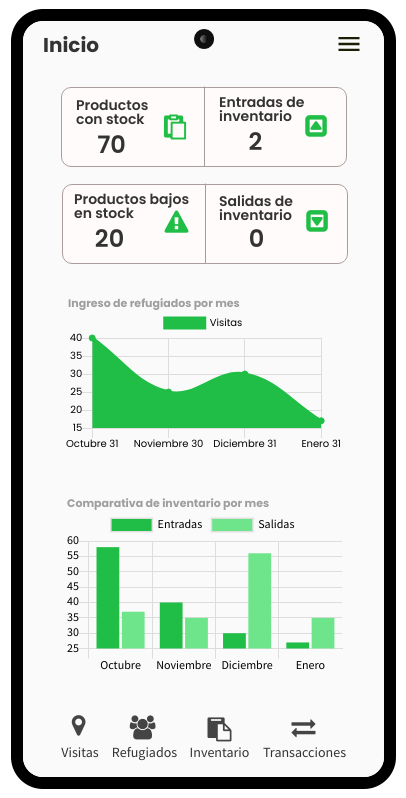
\includegraphics[width=3cm]{Inicio}
    \caption{Dashbooard}
\end{figure}
The user will be able to register and manage migrant data (view figure 3.3), subject to their system permissions. They can query this data and view each migrant's shelter entry history, enabling them to track the individual's movements within the country (view figure 3.4).
\begin{figure}[H]
   \begin{minipage}{0.4\textwidth}
     \centering
     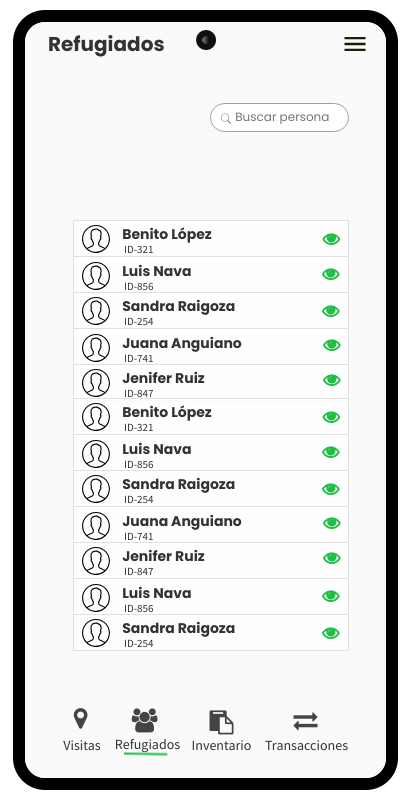
\includegraphics[width=.7\linewidth]{Refugiados}
     \caption{Migrants}\label{Fig:Data1}
   \end{minipage}\hfill
   \begin{minipage}{0.4\textwidth}
     \centering
     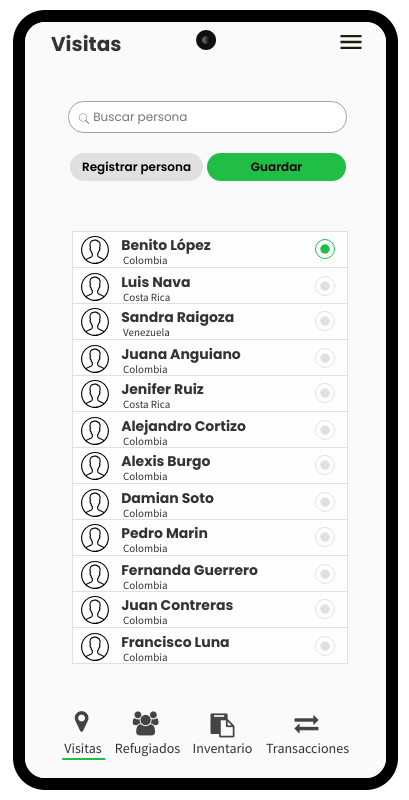
\includegraphics[width=.7\linewidth]{Visitas}
     \caption{Visits}\label{Fig:Data2}
   \end{minipage}
\end{figure}
Additionally, the user will have the capability to manage shelter resources, which includes accessing inventory details and conducting transactions (view figures 3.5 and 3.6).
\begin{figure}[H]
   \begin{minipage}{0.48\textwidth}
     \centering
     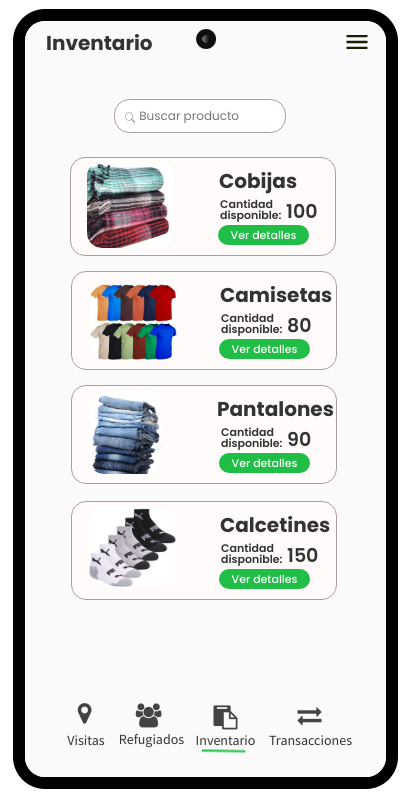
\includegraphics[width=.7\linewidth]{Inventario}
     \caption{Inventory}\label{Fig:Data1}
   \end{minipage}\hfill
   \begin{minipage}{0.48\textwidth}
     \centering
     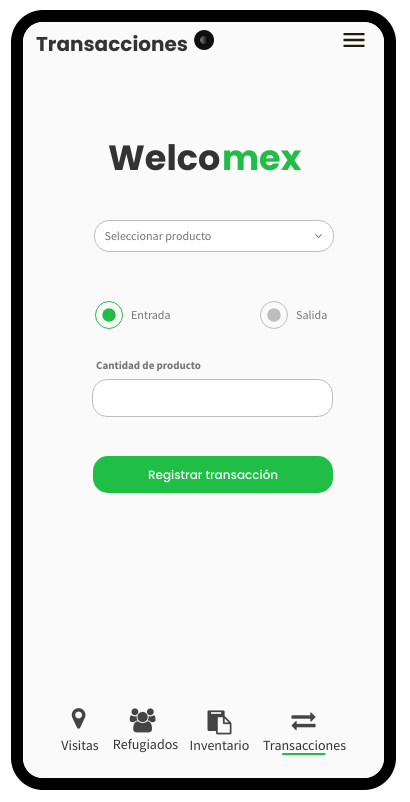
\includegraphics[width=.7\linewidth]{Transacciones}
     \caption{Add Transactions}\label{Fig:Data2}
   \end{minipage}
\end{figure}









\section{Hardware Interfaces}
The Welcomex system, primarily being a web-based application, minimizes the need for direct interaction with hardware components through its user-facing functionalities. However, its operations still entail certain interactions with hardware, both on the user end and within its cloud-based infrastructure. Herein, we outline the logical and physical characteristics of interfaces between the Welcomex software and the hardware components it interacts with.

\subsection*{Supported Device Types}
\begin{itemize}
    \item \textbf{Computers (Desktops and Laptops):} The system supports devices running major operating systems such as Windows, macOS, and Linux. These devices allow users to access the full range of functionalities offered by the Welcomex PWA through web browsers.
    \item \textbf{Mobile Devices (Smartphones and Tablets):} The PWA is designed to be fully functional on iOS and Android devices, ensuring users can access the application on the go. This includes data entry, consultation of dashboards, and other key functionalities.
\end{itemize}

\subsection*{Nature of Data and Control Interactions}
\begin{itemize}
    \item \textbf{Input Devices (Keyboard, Mouse, Touchscreen):} User interactions with the Welcomex system via input devices include data entry, navigation, and control commands within the PWA. The software is designed to respond to these inputs seamlessly, offering an intuitive user experience.
    \item \textbf{Cameras (For Facial Recognition):} In devices equipped with cameras, the software interfaces with the hardware to capture images for facial recognition purposes. This functionality requires the software to control the camera for capturing images, which are then processed by AWS Recognition services for identification or verification purposes.
    \item \textbf{Network Adapters (Wired and Wireless):} Communication with cloud-based services, including data storage and processing, is facilitated through the device's network adapters. The software relies on secure internet connections to exchange data with AWS services and other external APIs.
\end{itemize}

\section{Software Interfaces}
The Welcomex system is designed to integrate seamlessly with a variety of software components, leveraging their capabilities to enhance its functionalities. These integrations facilitate data exchange, processing, and storage, contributing to the system's efficiency and effectiveness. Below is an overview of the key software interfaces, the nature of the data exchanged, and the communications protocols involved.

\subsection*{Database Management System (DBMS)}
\begin{itemize}
    \item \textbf{Name and Version:} PostgreSQL, version 12. This choice is due to PostgreSQL's robustness, scalability, and support for complex queries, which are essential for handling the extensive migration data managed by Welcomex.
    \item \textbf{Data:} The system interacts with the database to query, insert, update, and delete data records, including migrant profiles, shelter inventories, and visit logs. These interactions are crucial for maintaining accurate and up-to-date information within the system.
    \item \textbf{Services:} The database provides storage and retrieval services, supporting complex queries that enable the analysis and visualization of migration data.
    \item \textbf{Nature of Communications:} Communications with the database occur through SQL queries, executed via the application's backend. The backend serves as an intermediary, processing requests from the frontend and translating them into database operations.
\end{itemize}

\subsection*{Cloud Services (AWS)}
\begin{itemize}
    \item \textbf{Integrated Components:} AWS S3 for data storage, AWS Recognition for facial recognition, and AWS Lambda for serverless computing.
    \item \textbf{Data:} Images and documents are stored in and retrieved from S3, facial recognition data is sent to and received from AWS Recognition, and Lambda functions are triggered for data processing tasks.
    \item \textbf{Services:} These AWS services provide scalable storage, advanced data processing capabilities, and facial recognition services, respectively.
    \item \textbf{Nature of Communications:} The system uses AWS SDKs and APIs for communication, adhering to RESTful principles for data exchange. Secure access is managed through AWS IAM roles and policies.
\end{itemize}

\subsection*{Operating Systems}
\begin{itemize}
    \item \textbf{Supported Systems:} The system is designed to be compatible with major operating systems, including Windows, macOS, Linux (for desktops), and iOS, Android (for mobile devices), ensuring broad accessibility.
    \item \textbf{Data:} Operating system compatibility affects the presentation and functionality of the PWA, as well as the integration with device hardware (e.g., cameras for facial recognition).
    \item \textbf{Services:} The primary service needed from the operating system is the support for modern web browsers, which are the primary interface for interacting with the Welcomex system.
\end{itemize}

\subsection*{Web Browsers}
\begin{itemize}
    \item \textbf{Supported Browsers:} Google Chrome, Mozilla Firefox, Safari, and Microsoft Edge. These browsers are required to support the latest web technologies used in the PWA, such as HTML5, CSS3, and JavaScript ES6+.
    \item \textbf{Data:} User interactions with the system, including data entry, queries, and navigation, are facilitated through the web browser.
    \item \textbf{Services:} Rendering of the PWA, execution of JavaScript for dynamic content and interactions, and secure communication over HTTPS.
\end{itemize}
Data sharing among these components is facilitated through API calls and database operations, adhering to a microservices architecture that ensures modularity and scalability. Sensitive data, particularly personal information about migrants, is encrypted in transit and at rest, with access controls implemented to protect privacy.

\section{Communications Interfaces}
The Welcomex system necessitates a comprehensive suite of communication interfaces to support its functionalities, ranging from user interactions through web browsers to secure data exchanges with cloud services and APIs. These communication requirements are crucial for ensuring efficient, secure, and reliable operations of the system. Below, we detail the key aspects of the communications interfaces required by the Welcomex system.
\subsection*{Web Browser Communication}
HTTPS (Hypertext Transfer Protocol Secure) is the primary protocol for web browser communication, ensuring secure access to the Welcomex PWA. HTTPS encrypts data in transit, protecting it from interception or tampering. Communication via web browsers utilizes standard web technologies, including HTML for content structure, CSS for presentation, and JavaScript for dynamic interactions and asynchronous data requests using Fetch API.
\subsection*{E-mail Notifications}
The system sends automated e-mail notifications for various purposes, such as alerting shelter managers and employees about stock levels, reminding users of upcoming events, or providing families with updates on migrant registrations.

SMTP (Simple Mail Transfer Protocol) is used for sending emails, with security enhancements such as SMTPS (SMTP Secure) or SMTP over TLS (Transport Layer Security) to encrypt email transmissions.
\subsection*{Network Server Communications}
In addition to HTTPS for web interactions, the system uses RESTful APIs for server communications with both internal components (e.g., between the front end and back end) and external services (e.g., cloud services, external databases). The system is designed to optimize data transfer rates through efficient API design and response caching. Synchronization mechanisms, such as webhooks or polling, are used to ensure data consistency across the system and with external interfaces.
\subsection*{Cloud Services Communication}
Communication with AWS services (e.g., S3 for storage, Recognition for facial recognition) uses AWS SDKs, which encapsulate the HTTPS-based API calls to these services. IAM (Identity and Access Management) roles and policies secure these communications. All communications with AWS services are encrypted using TLS, ensuring the confidentiality and integrity of data in transit.
\subsection*{Communication Security and Encryption}
All data in transit is encrypted using TLS, and sensitive data stored in the database or cloud storage is encrypted at rest. Secure access to the system and its data is managed through authentication mechanisms (e.g., OAuth 2.0, JWTs for API access) and authorization controls to ensure that users and systems have appropriate access levels.

These communication interfaces and protocols are integral to the functionality and security of the Welcomex system, ensuring that users can reliably and safely interact with the system, while also facilitating the secure and efficient exchange of data across the system's various components and with external services.

\chapter{System Features}
\section{Migrant Registration and Profile Management}
\subsection{Description and Priority}
This feature allows for the registration of migrants and the management of their profiles. It is of high priority due to its critical role in ensuring accurate data collection and assistance provision to migrants. The priority components are rated as follows: benefit (9), penalty (9), cost (5), risk (3).
\subsection{Stimulus/Response Sequences}
\begin{enumerate}
    \item \textbf{Stimulus:} A user selects the option to register a new migrant.
    \item \textbf{Response:} The system presents a form to enter migrant details.
    \item \textbf{Stimulus:} The user submits the completed registration form.
    \item \textbf{Response:} The system validates the data and creates a new migrant profile.
    \item \textbf{Stimulus:} The user edits an existing migrant profile.
    \item \textbf{Response:} The system updates the profile with the new information.
\end{enumerate}
\subsection{Functional Requirements}
\begin{enumerate}[label=REQ-\arabic*:,series=func-req, leftmargin=60pt]
    \item The system must allow users to enter detailed information about migrants, including name, age, nationality, and reason for migration.
    \item The system must validate the input data for completeness and format correctness.
    \item The system must provide an option to search for existing migrant profiles using name or facial recognition.
    \item The system must allow for the editing and updating of migrant profiles.
    \item In case of invalid inputs or system errors during registration, the system must display informative error messages guiding the user to correct the issue.
\end{enumerate}

\section{Data Visualization and Reporting}
\subsection{Description and Priority}
This feature provides dynamic dashboards for visualizing migration data and generating reports. It has a high priority for enabling decision-makers to understand migration trends and allocate resources effectively. The priority components are rated as follows: benefit (8), penalty (7), cost (4), risk (2).
\subsection{Stimulus/Response Sequences}
\begin{enumerate}
    \item \textbf{Stimulus:} A user accesses the dashboard to view migration statistics.
    \item \textbf{Response:} The system displays a series of interactive charts and graphs.
    \item \textbf{Stimulus:} The user selects specific criteria for data filtering.
    \item \textbf{Response:} The system updates the visualizations to reflect the selected filters.
    \item \textbf{Stimulus:} The user requests a report based on current dashboard data.
    \item \textbf{Response:} The system generates and downloads the report in the desired format.
\end{enumerate}
\subsection{Functional Requirements}
\begin{enumerate}[resume*=func-req, leftmargin=60pt]
    \item The system must provide interactive dashboards with real-time migration data.
    \item The system must allow users to customize data visualizations through filtering and sorting.
    \item The system must support the generation of reports in various formats (e.g., PDF, Excel).
    \item The system must ensure data privacy and security in reports and dashboards.
\end{enumerate}

\section{Shelter Inventory Management}
\subsection{Description and Priority}
Enables shelter managers and employees to track and manage inventory supplies. This feature is of medium priority, essential for the efficient operation of shelters. The priority components are rated as follows: benefit (7), penalty (6), cost (3), risk (4).
\subsection{Stimulus/Response Sequences}
\begin{enumerate}
    \item \textbf{Stimulus:} A user accesses the inventory management module.
    \item \textbf{Response:} The system displays current inventory levels and needs.
    \item \textbf{Stimulus:} The user updates inventory levels after receiving new supplies.
    \item \textbf{Response:} The system reflects the updated inventory status.
    \item \textbf{Stimulus:} The system detects low inventory levels.
    \item \textbf{Response:} The system alerts the user and suggests reordering.
\end{enumerate}
\subsection{Functional Requirements}
\begin{enumerate}[resume*=func-req, leftmargin=60pt]
    \item The system must allow users to input and update inventory items and quantities.
    \item The system must automatically alert users when inventory levels are low.
    \item The system must provide historical inventory usage data to aid in forecasting.
    \item The system must facilitate the generation of inventory reports and order lists.
\end{enumerate}

\section{User Access and Role Management}
\subsection{Description and Priority}
This feature enables the definition, assignment, and management of user roles and permissions within the Welcomex system. It is of high priority as it underpins the system’s security by ensuring that users have appropriate access levels based on their responsibilities. The priority components are rated as follows: benefit (9), penalty (8), cost (4), risk (5).
\subsection{Stimulus/Response Sequences}
\begin{enumerate}
    \item \textbf{Stimulus:} An administrator creates new user roles with specific permissions.
    \item \textbf{Response:} The system stores the new roles and their associated permissions.
    \item \textbf{Stimulus:} An administrator assigns a user role to a new or existing user.
    \item \textbf{Response:} The system updates the user’s access rights according to the assigned role.
    \item \textbf{Stimulus:} A user attempts to access a system feature outside their permissions.
    \item \textbf{Response:} The system denies access and optionally logs the attempt.
\end{enumerate}
\subsection{Functional Requirements}
\begin{enumerate}[resume*=func-req, leftmargin=60pt]
    \item The system must allow administrators to define and manage user roles and permissions.
    \item The system must enforce access controls based on user roles, restricting or granting access to specific features accordingly.
    \item The system must provide an audit trail of user actions, especially for access attempts and changes to roles or permissions.
    \item In case of unauthorized access attempts, the system must display an error message and notify administrators.
\end{enumerate}

\section{Facial Recognition for Migrant Identification}
\subsection{Description and Priority}
This feature integrates facial recognition technology to identify and verify migrants' identities, streamlining the registration and check-in processes at shelters. It's assigned a high priority due to its potential to enhance security and efficiency significantly. The priority components are rated as follows: benefit (8), penalty (7), cost (6), risk (4).
\subsection{Stimulus/Response Sequences}
\begin{enumerate}
    \item \textbf{Stimulus:} A user uploads a migrant's photo for identification.
    \item \textbf{Response:} The system processes the image using facial recognition technology and matches it with existing profiles.
    \item \textbf{Stimulus:} The system identifies a match or suggests potential matches.
    \item \textbf{Response:} The user reviews and confirms the match, updating or accessing the migrant's profile.
    \item \textbf{Stimulus:} No match is found.
    \item \textbf{Response:} The system prompts the user to create a new profile or retry with a different photo.
\end{enumerate}
\subsection{Functional Requirements}
\begin{enumerate}[resume*=func-req, leftmargin=60pt]
    \item The system must integrate with a facial recognition service (e.g., AWS Recognition) to process and match faces accurately.
    \item The system must securely handle and store biometric data in compliance with privacy regulations.
    \item The system must provide an interface for users to upload and verify photos against the database.
    \item The system must handle non-matches or ambiguous matches gracefully, providing options for user intervention.
\end{enumerate}

\chapter{Other Nonfunctional Requirements}
\section{Performance Requirements}
Performance requirements are essential to ensure that the Welcomex system meets the expectations of its users in terms of responsiveness, speed, and reliability. These requirements should be clearly articulated to guide the developers in creating an application that not only functions correctly but also delivers a seamless user experience. Here are some of the performance requirements that could be considered for the Welcomex system:

\begin{itemize}
    \item Fast response times are essential for user satisfaction and can significantly impact the perception of the application's quality.
    \item Efficient data processing and real-time synchronization ensure that the application supports a dynamic environment where timely information is critical.
    \item High system availability is a must-have for an application that supports essential services such as refugee management and support.
    \item The ability to handle a large number of user sessions is critical for scalability, particularly in scenarios of high demand or during crisis situations.
    \item Quick search functionality is vital for operational efficiency, especially when dealing with large amounts of data.
    \item Reliable facial recognition performance is critical for security and identification purposes.
    \item Robust backup and recovery capabilities are necessary to protect data integrity and ensure continuity of operations.
\end{itemize}

\section{Safety Requirements}
The safety strategy of Welcomex is characterized by specific requirements designed to safeguard the integrity and confidentiality of information. The implementation of daily automatic backups guarantees the availability and prompt recovery of data in adverse situations. Secure storage and strict compliance with privacy regulations in the areas of operation ensure the protection of sensitive data.
\begin{itemize}
    \item The system will perform automatic daily backups of all stored data, with the ability to recover information in case of loss or damage.
    \item A detailed logging system will be established for all user activities, enabling effective auditing to detect and address potential threats or unusual behavior.
    \item Welcomex will commit to comply with recognized security standards and relevant certifications in the field of data protection and information security management.
    \item All sensitive migrant and shelter data will be securely stored in compliance with privacy and data protection regulations in Welcomex geographic area of operation.
\end{itemize}

\section{Security Requirements}
Welcomex prioritizes security through a series of key requirements. Continuous security training is provided to ensure data integrity and minimize risk. Furthermore, commitments to regular software updates and adherence to security standards reinforce Welcomex's status as a trusted platform, aligning with the highest industry benchmarks.

\begin{itemize}
    \item A strong authentication system including two-factor verification will be implemented to reduce the risk of unauthorized access and safeguard data integrity.
    \item Regular training will be provided to users on secure practices, with the objective of avoiding actions that could result in data loss or compromise of system security.
\end{itemize}

\section{Software Quality Attributes}
Welcomex is dedicated on offering not just strong functionality but also an outstanding user experience. To achieve this goal, we have precisely outlined software quality attributes. These carefully crafted attributes aim to fulfill operational requirements and establish quality and performance benchmarks that surpass the expectations of our users and developers. 

\begin{itemize}
    \item \textbf{Adaptability:} Ability to quickly adjust to changes in requirements or operating environment.
    \item \textbf{Availability:} Guarantee of high operability and constant accessibility for authorized users.
    \item \textbf{Correctness:} Accuracy and precision in the execution of functionalities to validate data and guarantee efficiency.
    \item \textbf{Usability:} Intuitive and user-friendly interface, prioritizing a positive and efficient user experience.
    \item \textbf{Maintainability:} Ease of modifying, improving or correcting the system, ensuring continuous evolution.
    \item \textbf{Portability:} Adaptability to different environments and platforms without losing functionality.
    \item \textbf{Reliability:} Execution without critical errors, essential to maintain data integrity and service effectiveness.
\end{itemize}
\section{Business Rules}
The business rules set the essential guidelines for Welcomex's operation. They specify the permissions for various actions on the platform, ranging from registering shelters to updating migrant data. These rules create a robust framework to ensure legality, data security, and controlled information access, thus guaranteeing the system's effectiveness and reliability in fulfilling its humanitarian mission.

\begin{itemize}
    \item Shelter Registration: Only organizations or entities legally recognized as shelters can register on the platform.
    \item Migrant Registration: Migrant information can only be registered by authorized shelter staff.
    \item Access to Sensitive Data: Access to sensitive migrant data is restricted to authorized users, such as shelter staff and competent authorities.
    \item Data Consultation by Family Members: Family members of migrants may only consult specific information about their loved ones, and access is subject to identity verification.
    \item Updating Information: Data updates for both shelters and migrants can only be performed by authorized users to maintain the accuracy of the information.
    \item Regulatory Compliance: Welcomex will strictly follow the privacy and data protection regulations in force in the regions where it operates.
\end{itemize}

\chapter{Other Requirements}
These supplemental requirements enhance the Software Requirements Specification (SRS) by addressing key aspects that influence not only the system's functionality but also its security, legal compliance, and international adaptability.

\section*{Database}
A secure and scalable database is required, capable of effectively managing extensive migrant and shelter data. Regular backups of the database must be performed to ensure data integrity and availability.

\section*{Internationalization}
The user interface should be designed for multi-language support, offering an inclusive experience for users from various nationalities.

\section*{Legal}
The system must adhere to privacy and data protection laws in all regions where it operates, ensuring legal and ethical management of information.

\section*{Reusability}
The development of the system should promote the reuse of components and modules to optimize resources and ease future enhancements.

\addchap{Appendix A: Data Models}
\begin{figure}[H]
    \centering
    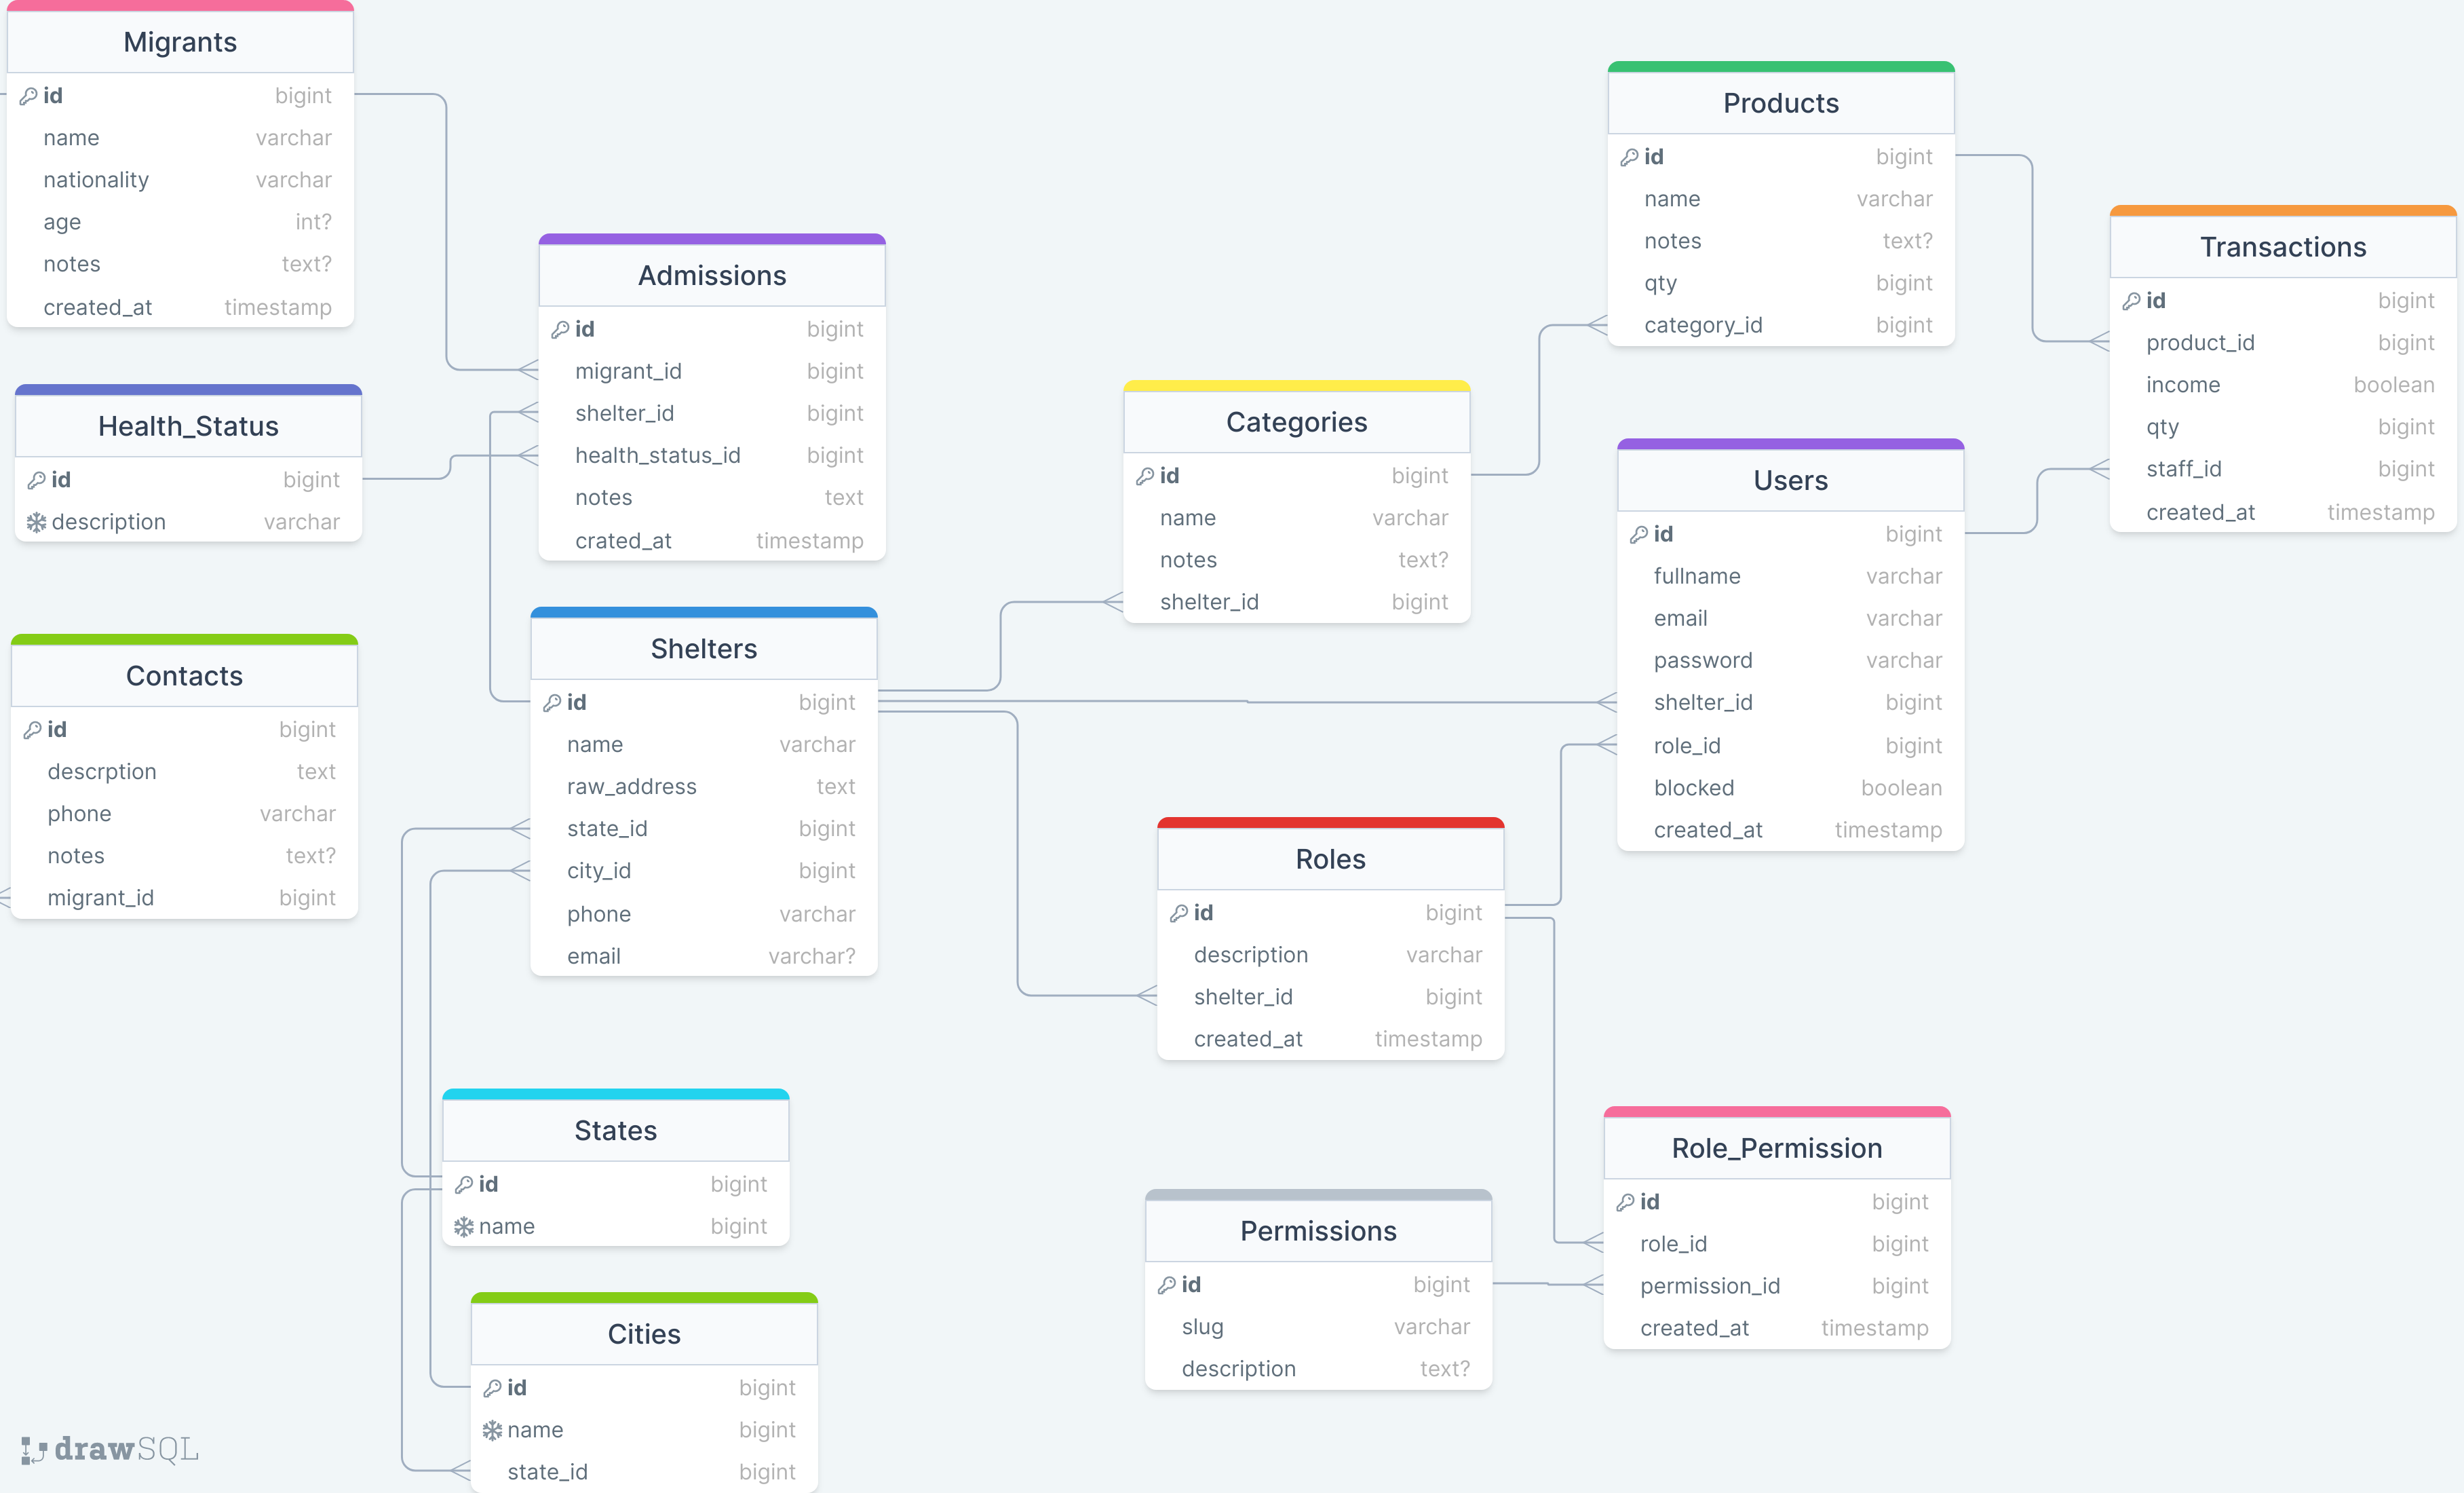
\includegraphics[width=1.3\textwidth, angle=90]{database-diagram}
    \caption{Database model}
\end{figure}

\section*{Data Dictionary}

\subsection*{Migrants}
\begin{tabular}{|m{2.5cm}|m{2.5cm}|m{6cm}|}
\hline
\textbf{Attribute} & \textbf{Data Type} & \textbf{Description} \\
\hline
id & bigint & Unique identifier for each migrant. \\
\hline
name & varchar & Name of the migrant. \\
\hline
nationality & varchar & Nationality of the migrant. \\
\hline
age & int? & Age of the migrant (optional). \\
\hline
notes & text? & Additional notes about the migrant (optional). \\
\hline
created\_at & timestamp & Record creation timestamp. \\
\hline
\end{tabular}

\subsection*{Health Status}
\begin{tabular}{|m{2.5cm}|m{2.5cm}|m{6cm}|}
\hline
\textbf{Attribute} & \textbf{Data Type} & \textbf{Description} \\
\hline
id & bigint & Unique identifier for each health status. \\
\hline
description & varchar & Description of the health status. \\
\hline
\end{tabular}

\subsection*{Contacts}
\begin{tabular}{|m{2.5cm}|m{2.5cm}|m{6cm}|}
\hline
\textbf{Attribute} & \textbf{Type} & \textbf{Description} \\
\hline
id & bigint & Unique identifier for each contact. \\
\hline
description & text & Description or type of contact (e.g., family, friend, lawyer). \\
\hline
phone & varchar & Contact phone number. \\
\hline
notes & text? & Additional notes or comments about the contact. \\
\hline
migrant\_id & bigint & Foreign key to the associated migrant. \\
\hline
\end{tabular}

\subsection*{Shelters}
\begin{tabular}{|m{2.5cm}|m{2.5cm}|m{6cm}|}
\hline
\textbf{Attribute} & \textbf{Type} & \textbf{Description} \\
\hline
id & bigint & Unique identifier for each shelter. \\
\hline
name & varchar & Name of the shelter. \\
\hline
raw\_address & text & The raw address information for the shelter. \\
\hline
state\_id & bigint & Foreign key to the associated state. \\
\hline
city\_id & bigint & Foreign key to the associated city. \\
\hline
phone & varchar & Contact phone number for the shelter. \\
\hline
email & varchar? & Contact email address for the shelter, if available. \\
\hline
\end{tabular}

\subsection*{Admissions}
\begin{tabular}{|m{2.5cm}|m{2.5cm}|m{6cm}|}
\hline
\textbf{Attribute} & \textbf{Type} & \textbf{Description} \\
\hline
id & bigint & Unique identifier for each admission record. \\
\hline
migrant\_id & bigint & Foreign key to the associated migrant. \\
\hline
shelter\_id & bigint & Foreign key to the associated shelter. \\
\hline
health\_status\_id & bigint & Foreign key to the associated health status. \\
\hline
notes & text & Additional notes or comments about the admission. \\
\hline
created\_at & timestamp & The date and time when the admission record was created. \\
\hline
\end{tabular}

\subsection*{Categories}
\begin{tabular}{|m{2.5cm}|m{2.5cm}|m{6cm}|}
\hline
\textbf{Attribute} & \textbf{Type} & \textbf{Description} \\
\hline
id & bigint & Unique identifier for each category. \\
\hline
name & varchar & Name of the category. \\
\hline
notes & text? & Additional notes or comments about the category. \\
\hline
shelter\_id & bigint & Foreign key to the associated shelter. \\
\hline
\end{tabular}

\subsection*{Products}
\begin{tabular}{|m{2.5cm}|m{2.5cm}|m{6cm}|}
\hline
\textbf{Attribute} & \textbf{Type} & \textbf{Description} \\
\hline
id & bigint & Unique identifier for each product. \\
\hline
name & varchar & Name of the product. \\
\hline
notes & text? & Additional notes or comments about the product. \\
\hline
qty & bigint & Quantity of the product available. \\
\hline
category\_id & bigint & Foreign key to the associated category. \\
\hline
\end{tabular}

\subsection*{Transactions}
\begin{tabular}{|m{2.5cm}|m{2.5cm}|m{6cm}|}
\hline
\textbf{Attribute} & \textbf{Type} & \textbf{Description} \\
\hline
id & bigint & Unique identifier for each transaction. \\
\hline
product\_id & bigint & Foreign key to the associated product. \\
\hline
income & boolean & Indicator of whether the transaction is an income (true) or expense (false). \\
\hline
qty & bigint & Quantity of the product transacted. \\
\hline
staff\_id & bigint & Foreign key to the associated staff member who handled the transaction. \\
\hline
created\_at & timestamp & The date and time when the transaction was recorded. \\
\hline
\end{tabular}

\subsection*{States}
\begin{tabular}{|m{2.5cm}|m{2.5cm}|m{6cm}|}
\hline
\textbf{Attribute} & \textbf{Type} & \textbf{Description} \\
\hline
id & bigint & Unique identifier for each state. \\
\hline
name & bigint & Name of the state. \\
\hline
\end{tabular}

\subsection*{Cities}
\begin{tabular}{|m{2.5cm}|m{2.5cm}|m{6cm}|}
\hline
\textbf{Attribute} & \textbf{Type} & \textbf{Description} \\
\hline
id & bigint & Unique identifier for each city. \\
\hline
name & bigint & Name of the city. \\
\hline
state\_id & bigint & Foreign key to the associated state. \\
\hline
\end{tabular}

\subsection*{Users}
\begin{tabular}{|m{2.5cm}|m{2.5cm}|m{6cm}|}
\hline
\textbf{Attribute} & \textbf{Type} & \textbf{Description} \\
\hline
id & bigint & Unique identifier for each user. \\
\hline
fullname & varchar & Full name of the user. \\
\hline
email & varchar & Email address of the user. \\
\hline
password & varchar & Encrypted password for user authentication. \\
\hline
shelter\_id & bigint & Foreign key to the associated shelter. \\
\hline
role\_id & bigint & Foreign key to the associated role. \\
\hline
blocked & boolean & Flag indicating whether the user is blocked from accessing the system. \\
\hline
created\_at & timestamp & The date and time when the user account was created. \\
\hline
\end{tabular}

\subsection*{Roles}
\begin{tabular}{|m{2.5cm}|m{2.5cm}|m{6cm}|}
\hline
\textbf{Attribute} & \textbf{Type} & \textbf{Description} \\
\hline
id & bigint & Unique identifier for each role. \\
\hline
description & varchar & Description of the role. \\
\hline
shelter\_id & bigint & Foreign key to the associated shelter. \\
\hline
created\_at & timestamp & The date and time when the role was created. \\
\hline
\end{tabular}

\subsection*{Permissions}
\begin{tabular}{|m{2.5cm}|m{2.5cm}|m{6cm}|}
\hline
\textbf{Attribute} & \textbf{Type} & \textbf{Description} \\
\hline
id & bigint & Unique identifier for each permission. \\
\hline
slug & varchar & Short, unique string identifying the permission, often used in code. \\
\hline
description & text? & A detailed description of what the permission allows. \\
\hline
\end{tabular}

\subsection*{Role\_Permission}
\begin{tabular}{|m{2.5cm}|m{2.5cm}|m{6cm}|}
\hline
\textbf{Attribute} & \textbf{Type} & \textbf{Description} \\
\hline
id & bigint & Unique identifier for each role\_permission association. \\
\hline
role\_id & bigint & Foreign key to the associated role. \\
\hline
permission\_id & bigint & Foreign key to the associated permission. \\
\hline
created\_at & timestamp & The date and time when the role\_permission association was created. \\
\hline
\end{tabular}

\addchap{Appendix B: Use Cases}


\end{document}